This chapter describes the process of desigining the molecule chip experiment.
This was motivated by three main factors: the need to integrate with the
existing experiment, the core proposal of confining molecules close to a
microwave guide, and the practicalities of fabricating the chip. Here I will
focus on how the first two factors informed the design choices, with changes
due to fabrication discussed in chapter~\ref{fab}. The design will be further
justified by simulation in chapter~\ref{design}.

We begin with a discussion of
the existing experiment, and where the chip fits into it. I will then discuss
the process that lead us to choose a magnetic trap for our design. I will
present the final design \cm{and how it can be integrated with the existing
apparatus}. 

\section{Existing \CaF{} apparatus}

\cm{Need to think a little about how this will build on theory chapter}

The methods for laser-cooling of molecules described in
chapter~\ref{theory} are applied in our experiments to produce cold \CaF{}
molecules. The apparatus shown in \myfigref{overview:fig:vacuumsystem} can be
used to produce and slow a \CaF{} beam~\cite{PhysRevA.89.053416, Truppe2017a}, capture these
molecules in a MOT and cool them below the Doppler limit~\cite{Truppe2017}. We
are then able to conduct experiments in coherent control of molecules in a
magnetic trap~\cite{PhysRevLett.124.063001} and investigate collisions with
rubidium atoms~\cite{PhysRevLett.126.153401, Jurgilas2021}.

\begin{figure}[htb]
  \centering
  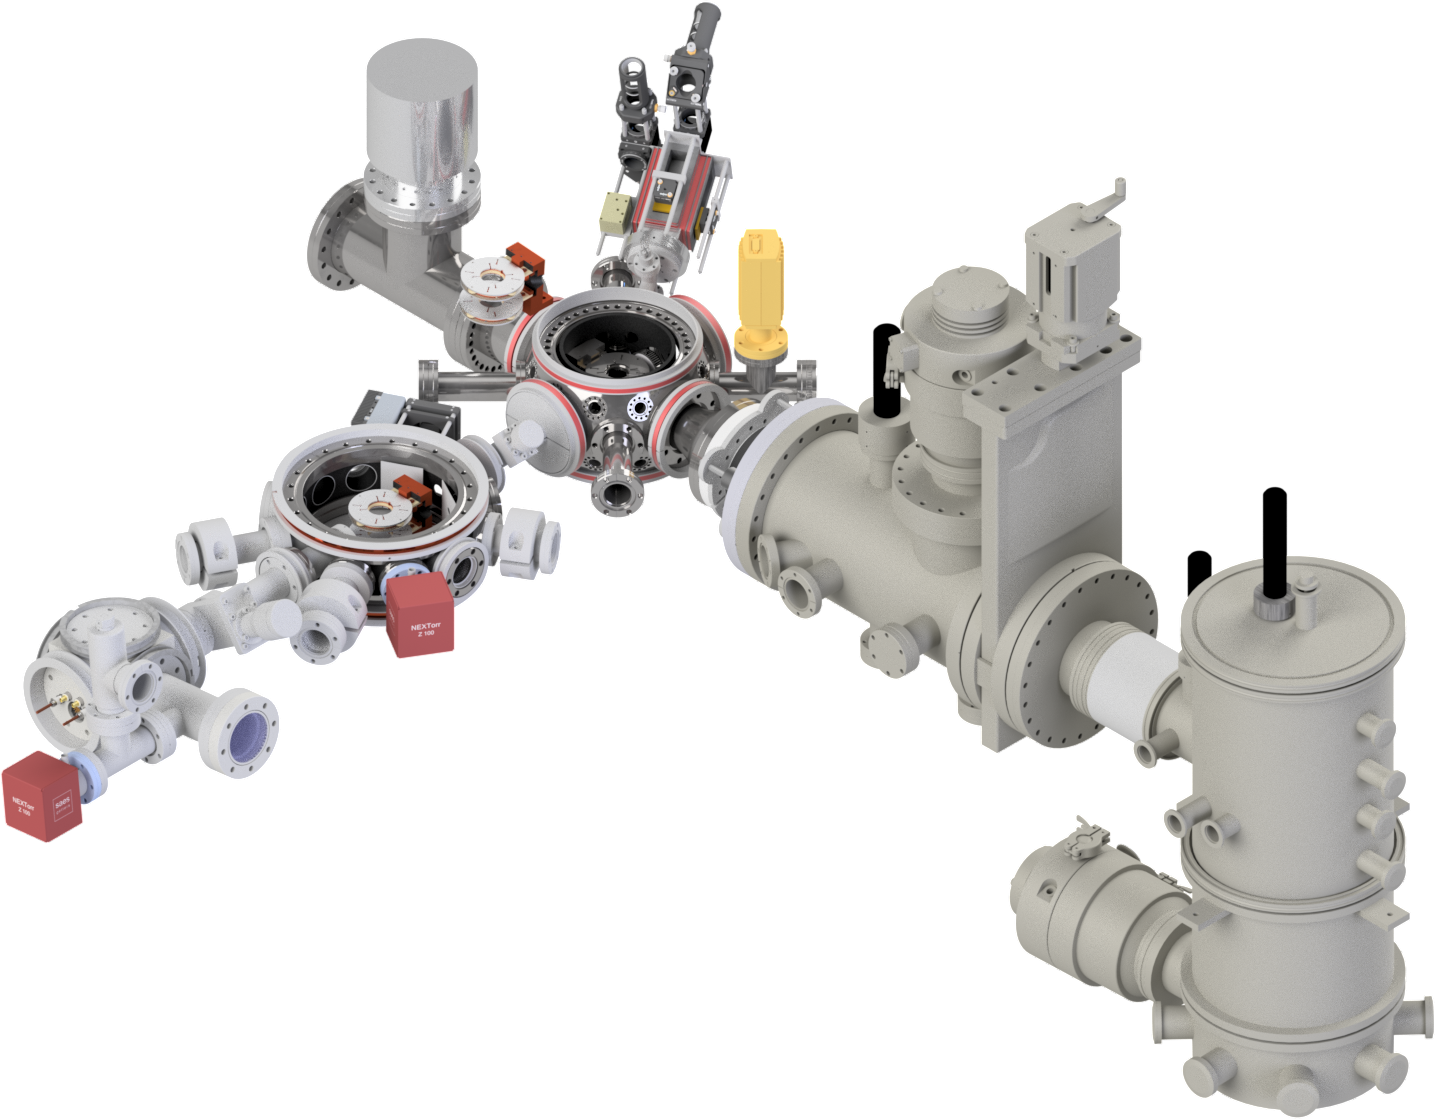
\includegraphics[width=0.7\textwidth]{figs/overview/apparatus_04_crp.png}
  \caption{
    The \CaF{} experiment is shown along with the planned additional chip
    chamber.}
  \label{overview:fig:vacuumsystem}
\end{figure}

All our experiments begin with the production of a beam of \CaF{} in the source
chamber with a buffer-gas cell. The molecules undergo laser-slowing before
being captured in a MOT in the MOT chamber. Subsequent experiments can be
conducted in this chamber or in the neighbouring tweezer chamber. This can be
populated by means of a magnetic transport trap (MTT).  Molecules can be
trapped in an external anti-Helmholtz coil mounted on a transport stage. Moving
the coils from their position around the MOT chamber can transport the trapped
molecules into the neighbouring tweezer chamber. \cm{To be discussed in later
chapter??}

The chip experiment will make use of this aparatus by adding an additional
experiment chamber downstream of the tweezer chamber, as shown in
\myfigref{overview:fig:vacuumsystem}. By transporting molecules through the
tweezer chamber and into this chip chamber, we will be able to load on to the
chip for this new experiment. In the rest of this chapter I will outline the
requirements for the chip experiment so that it can operate in conjunction with
the existing setup. I will then show how we have chosen to implement our
design.


\section{Design requirements}

\cm{
\begin{itemize}
  \item Andr\'e proposal, want to strongly couple to coplanar waveguides
  \item Wantto do quantum operations with rotational stretched states
  \item Need small size scale
  \item Height limited by VdW force, as per Ed's notebook (Charles Smith also said something
    about charges causing decoherence?) height gives scale size
  \item We want to use magnetic trapping rather than electric (as explained
    in QSUM report: long coherence times and easier to load (?))
  \item Need to be able to load (one step is no good, ref. next chapter)
\end{itemize}
}

\section{Design choices}
% TODO Maybe a better name for this 

\cm{
  \begin{itemize}
    \item Load with big U wire under chip
    \item IP better than QP because of majorana losses (so choose Z wires)
    \item Current and mw delivery by subchip (? this is a detail)
    \item Load via magnetic transport
  \end{itemize}
}

\section{Old stuff}
\label{overview:overview}

Our ultracold molecules are created using the methods described above, with our
apparatus, including the proposed chip chamber shown in
\myfigref{overview:fig:vacuumsystem}. A buffer-gas source is used to create
\CaF{} molecules in the source chamber, with the beam being longitudinally and
transversely slowed before it is captured in a MOT inside the collisions
chamber.


The \CaF{} MOT is the workhorse of our experiment, providing molecules which
can be further cooled cooled further (as discussed above) used for experiments
in collisions with \Rb{} atoms (see \inlinerefs{Jurgilas2021, JurgilasIOP2021,
PhysRevLett.126.153401}) and optical tweezers. The tweezer experiment is
undertaken in the neighbouring tweezer chamber, which is loaded by transporting
molecules in a magnetic transport trap (MTT), a quadrupole trap with coils
mounted on a transport stage outside the vacuum chamber. This transport of the
molecules is similar to that used in
\inlinerefs{Lewandowski2003,PhysRevResearch.1.033035} and elsewhere, it will be
discussed further below and in \cm{transport chapter}.

The chip experiment will integrate into this setup as shown in
\myfigref{overview:fig:vacuumsystem}, an additional chamber will be mounted
further downstream of the transport stage, so that molecules can be brought
straight through the tweezer chamber from the collisions chamber.  Since the
molecules will be brought into the chamber inside magnetic trap, we propose to
transfer them gradually into other magnetic traps formed on the chip.
%
Not only does this take advantage of the known, long-lived \CaF{} states in the
trap~\cite{WilliamsMagnetic2018}, but it allows us to follow the well-trodden
path of magnetic trapping near a chip, as has been outlined in previous
chapters.  The transfer to the chip will take the molecules through a series of
magnetic traps of decreasing size until they are in the smallest trap, similar
to what has previously been done in atom chips \cite{Reichel1999} or for
guiding molecules near surfaces \cite{Meek2009}

The chip will be held in its chamber recessed in a PCB used for power (and
later microwave) delivery. We use an aluminium-core PCB to ensure good heat
conduction away from the chip and we refer to it as the subchip.  This is
attached to a large copper heatsink, which has a large U-wire built into it,
isolated from the rest of the copper by aluminium-nitride plates. The heatsink
connects to a flange equipped with a \cm{?} pin feedthrough for chip currents,
and two high-current feedthroughs to power the U-wire.

% TODO Ensure I go on to discuss the current drivers
% TODO confirm distance in this para
We refer to this entire device as the flange assembly, and it is shown in the
inset of \myfigref{overview:fig:vacuumsystem} and in
\mysubfigref{overview:fig:chipexperiment} It will be mounted so that the chip is
\SI{3}{\milli\meter} away from the transport axis and facing the floor,
allowing us to trap and then drop the molecules for imaging.  External magnetic
coils will provide the bias fields, and currents will be provided by drivers
discussed in \cm{a later chapter.} {a}.

\begin{figure}[ht]
  \centering
  \begin{subfigure}[b]{0.45\textwidth}
    \includegraphics[width=\textwidth]{figs/chip_pic_crop.png}
    \caption{}
  \end{subfigure}
  \hspace{1cm}
  \begin{subfigure}[b]{0.45\textwidth}
    \centering
    %\includegraphics[width=\textwidth]{figs/chip_present2.pdf}
    \begin{overpic}[abs, width=\textwidth]{figs/chip_present4.pdf}
      \put(10, 160){\small (i)}
      \put(60, 160){\small(ii)}
      \put(175, 60){\small(iv)}
      \put(110, 137){\small(iii)}
      \put(70, 90){\small \SI{20}{\micro\meter}}
      \put(112, 93){\small\SI{10}{\micro\meter}}
      \put(8, 42){\small $\mathrm{Z_0}$}
      \put(8, 10){\small $\mathrm{Z_1}$}
      \put(8, 200){\small $\mathrm{Z_2}$}
    \end{overpic}
    \caption{}
  \end{subfigure}
  \caption{
    In (a) we have the chip assembly fully constructed, with a view of the
    aluminium-core PCB (subchip) for current delivery. Note also the polyimide
    bushings to electrically isolate the retaining screws from the surface. The
    microwave feedthroughs remain disconnected. In (b) we show a schematic of
    the chip features, with the scaling exaggerated for visibility. The three
    overlapping Z-wires are shown and labeled. The gaps between the wires are
    highlighted.
    %
    Toward the left (i) is the
    electroplating connection pad and various features used for
    characterisation (ii). On Z2 it is possible to see several small pads used
    as anchors, to secure the thin wire to the substrate.  The axis of the
    $\mathrm{Z1}$ wire is labeled for reference (iii) and the other wires are
    similar. All of the above features  will be discussed further in
    chapter~\ref{fab}. The crest of Imperial College London (iv) is also
    included.}
  \label{overview:fig:chipexperiment}
\end{figure}

% TODO Check what these equations that I use actually are and where they go. I
% think the current wording might basically be the same equation twice...
The first stage of the magnetic transfer is to take the molecules from the MTT
to the large U-wire embedded in the heat sink.  The idea is to use this as a
deep, macroscopic trap that is well-aligned with the chip by virtue of being
built into the assembly, and can be easily aligned with the MTT, similarly to
other experiments such as \inlineref{Ott2001}.  Since it is under the chip, it
will of course be further from the molecule cloud than the other wires, hence
more current will be required to create a deep trap (as per
equations~\ref{intro:eq:trapbias} and~\ref{intro:eq:trapdepth}). The current is
limited to \SI{100}{\ampere} by the vacuum feedthroughs, allowing for a trap of
depth around \SI{2}{\milli\kelvin} by equation \cm{ref. earlier chapter}.

Once loaded into the U-trap, the molecules will be transferred through the
Z-wire traps on the chip. Each Z-wire should be sufficiently
large to maintain the currents required to form a trap at height $z$ below the
trap, whilst having a width and height  $w, h \ll z$ so that that the current
is highly localised compared to the cloud size.  This follows the widely-made
assumption in the literature that the trapping currents are carried by wires
which are infinitesimally small compared to the length scale of the trap
~\cite{2011Ac}.

% TODO Make sure that this link to fab chapter is ok
In the case of the first Z-wire, the molecules are still \SI{3}{\milli\meter}
away from the trapping wire. If we demand a trap depth of
$k_B\times\SI{1}{\milli\kelvin}$, then we will require a trapping current of
\SI{30}{\ampere} to form a trap of this depth.  We will discuss in
chapter~\ref{fab} that the maximum wire height that can reliably be fabricated
is \SI{5}{\micro\meter}, and we expect that the wires will be able to carry a
maximum current density of \SI{6E10}{\ampere\per\meter\squared}, as was found
for a similar chip design in \inlineref{Treutlein2008}. The Z-wire will
therefore have a width $w=\SI{200}{\micro\meter}$. Other wire parameters are
shown in \mytableref{overview:table:wires}.

The axial length of the wires also decreases to gradually reduce the size of
the trapped cloud in the $x$ direction. An exaggerated schematic of the wire
layout is shown in \myfigref{overview:fig:chipexperiment} and further details are
outlined in \mytableref{overview:table:wires}. All wires have been designed to
carry twice the current that is required in the loading scheme, so that there
is sufficient headroom for further experiments, and to reduce risk of
accidental damage to the chip during normal operation.

% TODO Maybe need more detail here
\begin{table}
  \centering
\begin{tabular}{lrrrrr}
  Name & Axis length (\si{\milli\meter}) & Width (\si{\micro\meter})& $I_\text{max}$ & Trap height (\si{\micro\meter}) \\
 \hline
  U & 16 & N/A& 100 & 3000\\
  $\mathrm{Z0}$ & 12 & 200& 60& $3000\rightarrow1000$ \\
  $\mathrm{Z1}$ &  6 & 20& 6& $1000\rightarrow100$ \\
  $\mathrm{Z2}$ &  2 & 2& 0.6& $100\rightarrow10$ \\
 \hline
\end{tabular}
  \caption{Details on the wire dimensions, maximum current, and desired
  trapping heights. The wire design is shown in
  \mysubfigref{overview:fig:chipexperiment}{c}. Note that the U-wire current is
  limited by vacuum feedthroughs and not by the maximum current calculated by
  the wire dimensions.  The maximum currents have been designed for use at only
  50\% of their potential maximum ($I_\text{max}$).
  }
  \label{overview:table:wires}
\end{table}

Each Z-trap will begin trapping at one height before the bias field is
increased to bring the trap centre closer to the surface (as per
% TODO back to link
%\myeqref{intro:eq:trapbias}
\cm{reference eqn. $B = \mu_0 I / (2\pi h)$}
).  To distinguish between the two trap stages for
each wire, we label them $\mathrm{ZX_i}$ for the initial (higher) trap and
$\mathrm{ZX_f}$ for the final (lower) trap, with $\mathrm{ZX}$ corresponding to
the wire labels in \mytableref{overview:table:wires}.

In order to incorporate microwave guides onto the chip. This can be
accomplished by adding an insulating layer on top of the wires, on to which we
can fabricate coplanar waveguides~\cite{1127105}. The flange has been designed
with microwave feedthroughs, so that microwaves can be launched onto the
subchip and carried to the chip via coplanar waveguides \cm{to be discussed in
a later chapter}.

Having broadly outlined the experiment, the rest of this chapter will justify
the design of the trapping wires by means of simulation and analysis
of the trapping potentials.

